\documentclass[11pt,a4paper,twocolumn]{article}
\usepackage[utf8]{inputenc}
\usepackage[utf8]{inputenc}
\usepackage[T1]{fontenc}
\usepackage[english]{babel}
\usepackage[document]{ragged2e}
\usepackage{multicol} 
\usepackage{vmargin}
\usepackage{graphicx}
\usepackage{listings}
\usepackage{natbib}

\setpapersize{A4}
\setmargins{1.65cm}       
{1.78cm}                      
{16.5cm}                     
{23.42cm}                   
{5pt}                           
{1cm}                         
{0pt}                           
{2cm}                         

\title{Cap with gps positioning sensors and obstacle detection system}
\author{
\small{First A. Author, Julio Bodero, Second A. Author,Karla Bowen} \\
\small{Third A. Author,Jocelyn Miranda,Fourth A. Author,Paul Sanchez}\\
\small{fifth A. Author,Jean Vera}}
\date{January 2019}
\begin{document}
\maketitle

\textit{Abstract- 
The following prototype was born to help blind people  
who require a cane to guide their touch and predict 
if there is a bump, a stone or a hole. What our group 
has proposed is to reduce the risk of these vulnerable
people and manufacture caps that will have: distance sensors 
and GPS positioning, for this the prototype will 
be developed in a Raspberry and using codes in C;
}
\justify


\section{Introduction}

Global Positioning System (GPS) makes use of signals sent by satellites in space and ground stations on Earth to accurately determine their position on Earth.
Radio Frequency signals sent from satellites and ground stations are received by the GPS. GPS makes use of these signals to determine its exact position.
The GPS itself does not need to transmit any information.
The signals received from the satellites and ground stations contain time stamps of the time when the signals were transmitted. By calculating the difference between the time when the signal was transmitted and the time when the signal was received. Using the speed of the signal, the distance between the satellites and the GPS receiver can be determined using a simple formula for distance using speed and time.
Using information from 3 or more satellites, the exact position of the GPS can be triangulated.

\section{Antecedent}
\subtitle{\textbf{Prototype}}
A prototype in software is a model of the behavior of the system that can be used to fully understand it or certain aspects of it and thus clarify the requirements ... A prototype is a representation of a system, although it is not a complete system, it has the characteristics of the final system or part of them.

Nowadays the developers of these formal languages ​​are developing interactive environments that:

Allow the analyst to interactively create a specification based on the language of a system or software.
Invoke automatic tools that translate the specification based on the executable code language.
Allow the customer to use the executable code of the product to refine the formal requirements.
Methods and tools for the development of prototypes, for the selection of an appropriate approach to prototype creation.\\

\subtitle{
\textbf{Raspberry Pi
}} 

is a low-cost computer, single-board computer or low-cost single-board computer (SBC) developed in the United Kingdom by the Raspberry Pi Foundation, with the aim of stimulating computer education in schools.

Although it is not expressly indicated if it is free hardware or with trademark rights, on its official website they explain that they have distribution and sale contracts with two companies, but at the same time anyone can become a reseller or re-distributor of the Raspberry Pi cards, 8 So it implies that it is a product with registered ownership, maintaining control of the platform, but allowing its free use both educationally and privately.
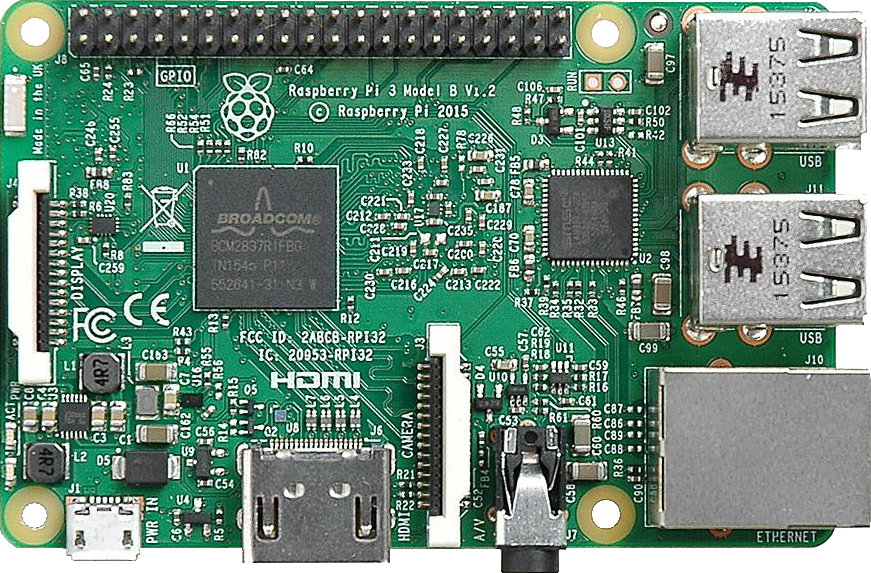
\includegraphics[width=230]{Raspberry_Pi_3_Model_B}


\subtitle{
\textbf{GNU/Linux,}
} 
also known as Linux, is a free Unix-like operating system; multiplatform, multiuser and multitasking. The system is the combination of several projects, among which stand out GNU (headed by Richard Stallman and the Free Software Foundation) and the Linux kernel (headed by Linus Torvalds). Its development is one of the most prominent examples of free software: all its source code can be used, modified and redistributed freely by anyone, under the terms of the GPL (GNU General Public License) and another series of free licenses.

\section{Development of the concept}

\subtitle{
\textbf{GPS system}
}

GPS refers to the acronym Global positioning system or Global Positioning System. This system is made up of many satellites that are kilometers away from the Earth's atmosphere and that are continuously sending signals to the Earth through radio frequencies. Our GPS module is a GPS receiver, the antenna that has received signals from the satellites that are around the Earth. It is necessary that at least receive a signal from 4 satellites to give a precise positioning. However, the receivers also have mathematical algorithms included that make the necessary calculations to subtract the difference of time it takes the signal to arrive and calculate the time and the correct distance in which the GPS receiver is located.

For better positioning accuracy, so-called control segments that are stations on the ground that communicate with the satellite network are usually used. Our GPS module uses the assisted GPS system to improve accuracy. This system uses the control segments to help GPS receivers to get more accurate and faster information from the satellite by providing the receiver with the appropriate data and accurate time, or by using its good signal and high processing power to interpret the broken or fragmented information that reaches the receiver. The assisted GPS system is the most used in mobile phones or mobile devices, and that is why they tend to have a better GPS signal than a GPS system alone.
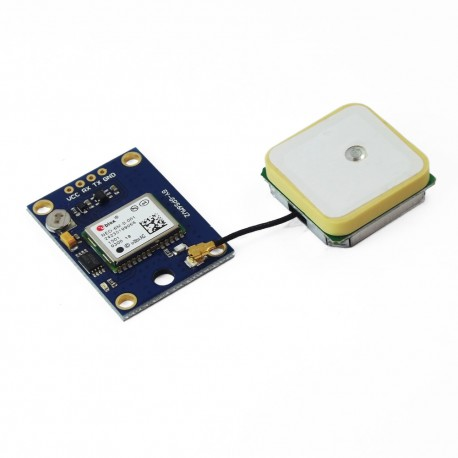
\includegraphics[width=230]{modulo-gps}

\subtitle{
\textbf{Wearable technology }
}
Body technology, technological clothing, 1 smart clothing, 2 wearable technology, 3 wearable or smart accessories, within the technology sector, and more specifically consumer electronics, is that electronic device that is worn on, under or included in the clothes. Another of its characteristics is that it allows multitasking so it does not require to stop doing something else to be used and can act as an extension of the user's body or mind.4 5 6

Wearable devices like activity monitors are a good example of the Internet of things, since things like electronics, software, sensors and connectivity are mechanisms that allow objects to exchange information through the Internet with a manufacturer, operator or others. connected devices, without needing human intervention.

Nowadays, the most important category of wearable devices is that of smart watches, followed by the categories of activity wristbands and smart glasses. According to its use can be divided into five large groups: 7

Health
Sport and wellness
Entertainment
Industrial
Military

\section{Implementation design}

\subtitle{
\textbf{Code used}
}
The following code was used to 
obtain the geo location data of the gps module
\begin{lstlisting}
import serial
#import RPi.GPIO as GPIO
import os, time
from decimal import *
delay = 1
#GPIO.setmode(GPIO.BOARD)
def find(str, ch):
for i, ltr in enumerate(str):
if ltr == ch:
yield i
port = serial.Serial("/dev/ttyAMA0"
, baudrate=9600, timeout=1)
cd=1
try:
while cd <= 50:
ck=0
fd=''
while ck <= 50:
rcv = port.read(10)
fd=fd+rcv
ck=ck+1
if '$GPRMC' in fd:
ps=fd.find('$GPRMC')
dif=len(fd)-ps
if dif > 50:
data=fd[ps:(ps+50)]
print(data)
p=list(find(data, ","))
lat=data[(p[2]+1):p[3]]
lon=data[(p[4]+1):p[5]]
s1=lat[2:len(lat)]
s1=Decimal(s1)
s1=s1/60
s11=int(lat[0:2])
s1=s11+s1
s2=lon[3:len(lon)]
s2=Decimal(s2)
s2=s2/60
s22=int(lon[0:3])
s2=s22+s2
print("Latitude:",s1)
print("Longitude:",s2)
cd=cd+1
print(cd)
except KeyboardInterrupt:
print("Thank You")
\end{lstlisting}

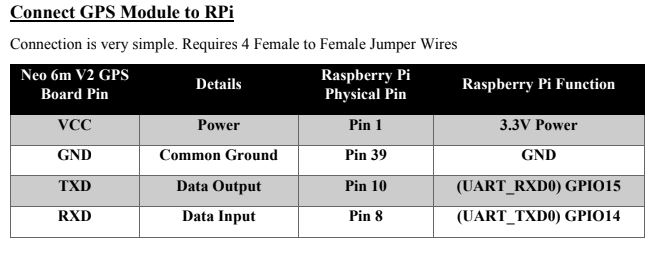
\includegraphics[width=260]{Captura}

\subtitle{
\textbf{Data Base}
}
You can use a database which recorded the location of the person the precision, and if in that location there is a collision that road is marked as a possible collision and passed to the next, so that the route traced by the device is the most optimal it is necessary that the device learn all the possible coordinates and verify all the collisions that can be made

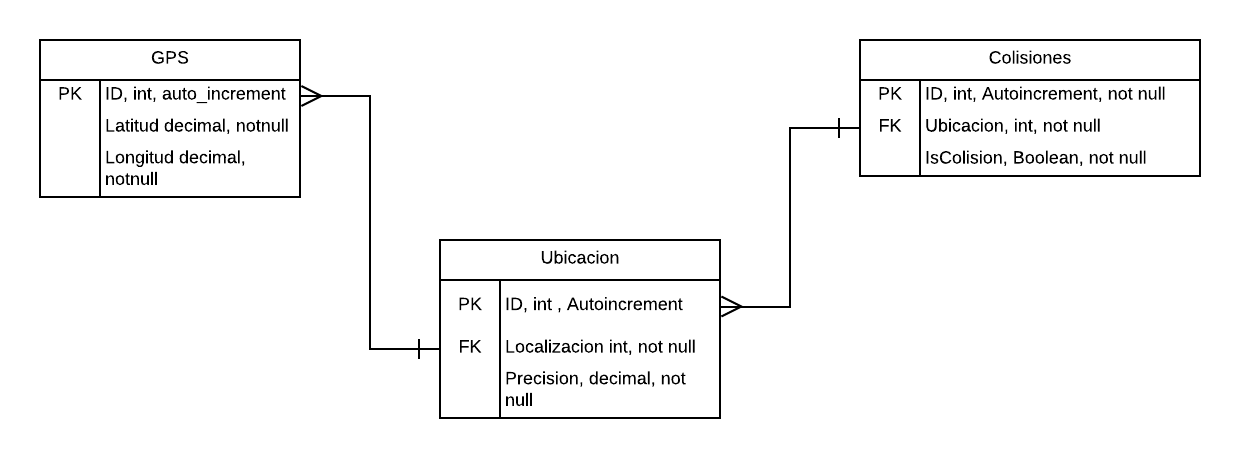
\includegraphics[width=230]{database}

\subtitle{
\textbf{Distance Sensor}
}
SRF04 is an ultrasonic distance sensor capable of detecting objects and calculating the distance to which it is in a range of 3 to 300 cm. The sensor works by ultrasound and contains all the electronics responsible for making the measurement. Its use is as simple as sending the start pulse and measuring the width of the return pulse. Of very small size, SRF04 stands out for its low consumption, high precision and low price so it is replacing the Polaroid sensors in the latest robots.
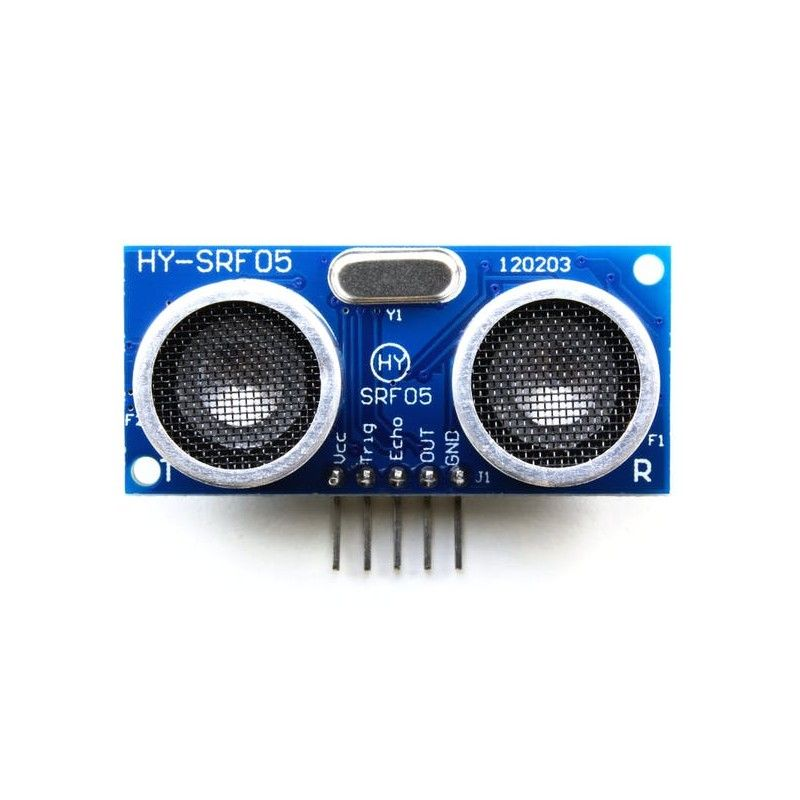
\includegraphics[width=230]{sensor}
\section{Conclusions}
- It is important that the database has many measurements of the latitude and longitude of our location so we must use a sample of about 10,000 data to make the location very accurate.
-Artificial intelligence algorithms must be implemented so that the device learns with the collisions found and in this way seek better routes without \\
-It is possible to implement projects made in arduino on a raspberry platform\\
-The cost of each attachment or sensor that is required for implementation are expensive.

\section{Recommendations}
-It takes more time, practice and knowledge about microprocessors and c language to be able to perform better projects\\
-Knowledge of C language and python is required to carry out implementations, in addition to knowledge of microprocessors
\section{References}
[1] Miguel Catalina Gallego; Alfredo Catalina Gallego
McGraw-Hill / Interamericana de España, S.A.
1. ed.(11/1998)
[2] RASPBERRY PI: Guía paso a paso para dominar 
El Hardware y Software de Raspberry PI 3
[3] nivar, chaves (2011). Curso de informática básica. En http://www.monografias.com/trabajos11/curinfa/curinfa.shtml 
(descarga el 8 de Octubre del 2011).
[4] Elkner, J., Downey, A. B. & Meyers, C. (2010). 
How to think like a computer scientist: Learning with Python. (2da. ed.) 
\end{document}

